% !TEX program = xelatex
% Rapport du projet One Look. Compiler avec XeLaTeX (deux passes), images dans img/.
\documentclass[10pt,a4paper]{article}
\usepackage{amsmath,amssymb,mathtools}
\usepackage{fontspec}
\usepackage{polyglossia}\setmainlanguage{french}
\usepackage[margin=2cm,top=2.2cm,bottom=2.2cm,headheight=14pt]{geometry}
\usepackage{microtype}
\usepackage[most]{tcolorbox}
\usepackage{tikz}
\usetikzlibrary{arrows.meta,calc,decorations.pathreplacing,positioning,fadings,shapes.geometric,shadows.blur}
\usepackage{pgfplots}
\pgfplotsset{compat=1.18}
\usepackage{enumitem,fancyhdr,titlesec,booktabs,tabularx,array,multicol,xcolor,graphicx,colortbl}
\usepackage[colorlinks=true,linkcolor=ink,urlcolor=sysblue]{hyperref}
\newcommand{\matiere}{ONE LOOK · RAPPORT DE PROJET}

% ---- Typographie
\setmainfont{Inter}[Extension=.otf,UprightFont=*-Regular,BoldFont=*-SemiBold,ItalicFont=*-Italic,BoldItalicFont=*-SemiBoldItalic,Numbers={Lining,Proportional}]
\setsansfont{Inter}[Extension=.otf,UprightFont=*-Regular,BoldFont=*-SemiBold,ItalicFont=*-Italic,BoldItalicFont=*-SemiBoldItalic]
\setmonofont{Inter}[Extension=.otf,UprightFont=*-Regular,Scale=0.92]
\IfFontExistsTF{InterDisplay-Bold.otf}{\def\dispname{InterDisplay}}{\def\dispname{Inter}}
\newfontfamily\displayfont{\dispname}[Extension=.otf,UprightFont=*-Bold,BoldFont=*-ExtraBold,LetterSpace=-2.2]
\newfontfamily\titlefont{\dispname}[Extension=.otf,UprightFont=*-SemiBold,BoldFont=*-Bold,LetterSpace=-1.2]
\newfontfamily\eyebrowfont{Inter}[Extension=.otf,UprightFont=*-SemiBold,LetterSpace=8]
\newfontfamily\captionfont{Inter}[Extension=.otf,UprightFont=*-Medium,ItalicFont=*-MediumItalic,LetterSpace=1.5]
\usepackage[italic,defaultmathsizes]{mathastext}
\linespread{1.18}

% ---- Couleurs
\definecolor{ink}{HTML}{1D1D1F}\definecolor{ink2}{HTML}{6E6E73}\definecolor{ink3}{HTML}{8E8E93}
\definecolor{separator}{HTML}{E5E5EA}\definecolor{fill}{HTML}{F5F5F7}\definecolor{fondgris}{HTML}{F2F2F5}
\definecolor{sysblue}{HTML}{007AFF}\definecolor{sysgreen}{HTML}{248A3D}\definecolor{sysorange}{HTML}{C93400}
\definecolor{sysred}{HTML}{D70015}\definecolor{syspurple}{HTML}{8944AB}\definecolor{systeal}{HTML}{0071A4}
\definecolor{sysindigo}{HTML}{5856D6}\definecolor{lightblue}{HTML}{EEF5FF}
\definecolor{eau}{HTML}{2F6DB3}\definecolor{feu}{HTML}{E0702A}\definecolor{fieldcol}{HTML}{FF9500}
\color{ink}

% ---- Titres
\setcounter{secnumdepth}{2}\setcounter{tocdepth}{1}
\newcommand{\chapeyebrow}{}
\newcommand{\chapitre}[3]{\clearpage\renewcommand{\chapeyebrow}{#1}%
  \refstepcounter{section}\setcounter{subsection}{0}\addcontentsline{toc}{section}{#1 · #2}%
  \vspace*{0.6cm}{\eyebrowfont\footnotesize\color{sysblue}\MakeUppercase{#1}\par}\vspace{6pt}
  {\displayfont\fontsize{34}{37}\selectfont\color{ink}#2\par}\vspace{8pt}
  {\titlefont\fontsize{14}{18}\selectfont\color{ink2}#3\par}\vspace{18pt}}
\renewcommand{\thesubsection}{\arabic{subsection}}
\titleformat{\subsection}{\titlefont\fontsize{17}{21}\selectfont\color{ink}}{\textcolor{sysblue}{\thesubsection}}{0.55em}{}
\titlespacing*{\subsection}{0pt}{20pt}{8pt}

% ---- En-tête / pied
\pagestyle{fancy}\fancyhf{}
\fancyhead[L]{\eyebrowfont\scriptsize\color{ink3}\matiere}
\fancyhead[R]{\captionfont\scriptsize\color{ink3}\chapeyebrow}
\fancyfoot[C]{\captionfont\scriptsize\color{ink3}\thepage}
\renewcommand{\headrulewidth}{0pt}
\setlist{itemsep=3pt,topsep=4pt,leftmargin=1.4em}\setlist[itemize]{label={\color{ink3}\textbullet}}
\setlength{\parindent}{0pt}\setlength{\parskip}{5pt}

% ---- Cartes (couleur = sens)
\tcbset{card/.style={enhanced,breakable,frame hidden,boxrule=0pt,arc=3.4mm,left=12pt,right=12pt,top=9pt,bottom=10pt,
  fonttitle=\eyebrowfont\scriptsize,titlerule=0pt,toptitle=9pt,bottomtitle=-3pt,lefttitle=12pt,before skip=10pt,after skip=10pt,
  fuzzy shadow={0mm}{-0.7mm}{-0.4mm}{1.1mm}{black!16!white}}}
\newcommand{\cardtitle}[1]{\MakeUppercase{#1}}
\newtcolorbox{definition}[1][]{card,colback=lightblue,colbacktitle=lightblue,coltitle=sysblue,title={\cardtitle{Cadrage}},#1}
\newtcolorbox{exemple}[1][]{card,colback=systeal!6,colbacktitle=systeal!6,coltitle=systeal,title={\cardtitle{Exemple}},#1}
\newtcolorbox{methode}[1][]{card,colback=sysgreen!6,colbacktitle=sysgreen!6,coltitle=sysgreen,title={\cardtitle{Correction apportée}},#1}
\newtcolorbox{astuce}[1][]{card,colback=fieldcol!9,colbacktitle=fieldcol!9,coltitle=sysorange,title={\cardtitle{Choix}},#1}
\newtcolorbox{attention}[1][]{card,colback=sysred!5,colbacktitle=sysred!5,coltitle=sysred,title={\cardtitle{Limite}},#1}
\newtcolorbox{retenir}[1][]{card,colback=syspurple!7,colbacktitle=syspurple!7,coltitle=syspurple,title={\cardtitle{À retenir}},fuzzy shadow={0mm}{-1mm}{-0.3mm}{1.6mm}{black!22!white},#1}
\newtcolorbox{complt}[1][]{card,colback=fill,colbacktitle=fill,coltitle=ink2,title={\cardtitle{Complément}},#1}
\newtcolorbox{codebox}[1][]{card,colback=fill,colbacktitle=fill,coltitle=ink2,title={\cardtitle{Terminal}},fontupper=\captionfont\footnotesize,#1}
\newcommand{\boxres}[1]{\begin{center}\tcbox[enhanced,frame hidden,colback=white,arc=2.6mm,boxrule=0pt,left=11pt,right=11pt,top=6pt,bottom=6pt,borderline west={2pt}{0pt}{sysblue},fuzzy shadow={0mm}{-0.6mm}{-0.2mm}{1.0mm}{sysblue!28!white}]{#1}\end{center}}
\newcommand{\chip}[2]{\tcbox[on line,enhanced,frame hidden,colback=#1!10,coltext=#1,arc=2mm,boxsep=1.5pt,left=5pt,right=5pt,top=1pt,bottom=1pt,fontupper=\eyebrowfont\tiny]{#2}}
\newcommand{\legende}[1]{\par\smallskip{\centering\captionfont\footnotesize\color{ink2}#1\par}\medskip}
\newcommand{\erreur}[2]{\item {\color{ink}#1}\newline{\color{sysgreen}\captionfont\small Correction\,: }#2}

% Grand chiffre de la page « En bref »
\newcommand{\chiffre}[3]{\begin{tcolorbox}[enhanced,frame hidden,boxrule=0pt,arc=3.4mm,colback=white,left=10pt,right=8pt,top=8pt,bottom=8pt,
  fuzzy shadow={0mm}{-0.7mm}{-0.4mm}{1.1mm}{black!14!white},equal height group=chiffres]
  {\displayfont\fontsize{30}{32}\selectfont\color{#1}#2\par}\vspace{4pt}{\captionfont\footnotesize\color{ink2}#3\par}\end{tcolorbox}}

% ---- Figures
\tikzset{>={Stealth[length=2.2mm,round]},every picture/.style={line cap=round,line join=round,font=\captionfont\small},
  boite/.style={draw=ink3,line width=0.6pt,rounded corners=2.4mm,fill=white,align=center,minimum height=1.35cm,text width=2.35cm,inner sep=4pt,font=\captionfont\scriptsize\color{ink2}},
  boiteforte/.style={boite,draw=sysblue,line width=1.2pt,fill=lightblue,font=\captionfont\scriptsize\color{ink}},
  fleche/.style={->,ink3,line width=0.7pt}}
\pgfplotsset{fiche/.style={axis lines=left,axis line style={ink3,semithick},tick style={ink3},
  grid=major,grid style={separator},tick label style={font=\captionfont\scriptsize,ink2},label style={font=\captionfont\small,ink2},
  title style={font=\titlefont\small,ink},
  legend style={font=\captionfont\scriptsize,draw=none,fill=white,fill opacity=0.92,text opacity=1,rounded corners=3pt}}}

\begin{document}

% =====================================================================
% COUVERTURE
% =====================================================================
\thispagestyle{empty}
\vspace*{0.4cm}
{\eyebrowfont\footnotesize\color{sysblue}PROJET D'IA EMBARQUÉE · NOVEMBRE 2026\par}\vspace{10pt}
{\displayfont\fontsize{64}{64}\selectfont\color{ink}One Look\par}\vspace{12pt}
{\titlefont\fontsize{17}{22}\selectfont\color{ink2}Détecter les inondations et les feux de forêt\\à bord d'un satellite, en une seule passe.\par}
\vspace{1.0cm}
\begin{center}
\begin{tikzpicture}
  % fond en dégradé
  \shade[left color=sysblue,right color=syspurple,middle color=sysindigo,rounded corners=6mm] (0,0) rectangle (16.5,7.2);
  % Terre (arc) et orbite
  \begin{scope}
    \clip[rounded corners=6mm] (0,0) rectangle (16.5,7.2);
    \fill[white,opacity=0.10] (8.25,-9.5) circle (11.2);
    \fill[white,opacity=0.10] (8.25,-9.5) circle (10.6);
    \draw[white,opacity=0.55,line width=0.8pt,dash pattern=on 4pt off 4pt] (8.25,-9.5) circle (13.3);
    % tuile observée au sol
    \begin{scope}[shift={(8.25,1.15)}]
      \fill[white,opacity=0.22,rounded corners=1mm] (-0.75,-0.45) rectangle (0.75,0.45);
      \draw[white,line width=0.9pt,rounded corners=1mm] (-0.75,-0.45) rectangle (0.75,0.45);
      \fill[eau!40,opacity=0.95] (-0.55,-0.2) .. controls (-0.2,0.25) and (0.1,-0.1) .. (0.55,0.2) -- (0.55,-0.3) -- (-0.55,-0.3) -- cycle;
    \end{scope}
    % faisceau
    \fill[white,opacity=0.16] (8.25,3.85) -- (7.5,1.6) -- (9.0,1.6) -- cycle;
    % satellite
    \begin{scope}[shift={(8.25,4.25)}]
      \fill[white] (-0.32,-0.24) rectangle (0.32,0.24);
      \fill[white,opacity=0.85] (-1.45,-0.17) rectangle (-0.48,0.17);
      \fill[white,opacity=0.85] (0.48,-0.17) rectangle (1.45,0.17);
      \draw[white,line width=0.8pt] (-0.48,0) -- (-0.32,0) (0.32,0) -- (0.48,0);
      \fill[sysindigo] (0,-0.24) circle (0.09);
    \end{scope}
    % décisions
    \node[white,font=\eyebrowfont\scriptsize] at (3.0,5.8) {INONDATION};
    \node[white,font=\eyebrowfont\scriptsize] at (13.5,5.8) {FEU};
    \node[white,font=\eyebrowfont\scriptsize,opacity=0.85] at (3.0,4.9) {NORMAL};
    \node[white,font=\eyebrowfont\scriptsize,opacity=0.85] at (13.5,4.9) {INCONNU};
    \node[white,font=\captionfont\footnotesize,opacity=0.9] at (8.25,6.55) {0,21 Mo · 4,8 ms par tuile · un seul cœur CPU};
  \end{scope}
\end{tikzpicture}
\end{center}
\vspace{0.6cm}
\begin{tcolorbox}[card,colback=fill,colbacktitle=fill,coltitle=ink2,title={\cardtitle{Comment lire ce rapport}}]
Chaque encadré a une couleur qui dit ce qu'il contient :
\chip{sysblue}{CADRAGE} règles du projet,
\chip{sysorange}{CHOIX} décisions techniques,
\chip{sysgreen}{CORRECTION APPORTÉE} solution à une erreur,
\chip{sysred}{LIMITE} ce qui ne marche pas encore,
\chip{syspurple}{À RETENIR} résultat clé,
\chip{ink2}{COMPLÉMENT} détails.
Les chiffres viennent du test, c'est-à-dire de pays jamais vus à l'entraînement. Code et données : \href{https://github.com/elrich-byte/one-look}{github.com/elrich-byte/one-look}.
\end{tcolorbox}

\clearpage
\thispagestyle{empty}
\vspace*{0.6cm}
{\eyebrowfont\footnotesize\color{sysblue}SOMMAIRE\par}\vspace{8pt}
{\displayfont\fontsize{34}{37}\selectfont\color{ink}Au programme\par}\vspace{20pt}
{\titlefont\large\renewcommand{\contentsname}{}\makeatletter\renewcommand\@pnumwidth{2em}\makeatother
\setlength{\parskip}{10pt}\tableofcontents}

% =====================================================================
\chapitre{En bref}{Objectif et résultat}{Un modèle de 0,21 Mo qui alerte peu, mais juste.}
% =====================================================================

Le modèle analyse une tuile Sentinel de 5 km sur 5 km et répond \textbf{INONDATION}, \textbf{FEU}, \textbf{NORMAL} ou \textbf{INCONNU}. Il tourne avec ONNX Runtime seul, comme il le ferait sur l'ordinateur de bord d'un satellite.

\begin{tcbraster}[raster columns=4,raster equal height=rows,raster column skip=8pt]
\chiffre{feu}{5\,\%}{de fausses alertes sur les images normales}
\chiffre{eau}{95\,\%}{des alertes inondation sont justes}
\chiffre{syspurple}{100\,\%}{des images inconnues testées sont signalées}
\chiffre{ink}{4,8 ms}{par tuile sur un seul cœur, pour 0,21 Mo}
\end{tcbraster}

\begin{definition}[title={\cardtitle{La question de recherche}}]
Après le point d'étape, l'encadrant a proposé une question : que perd-on avec une simple caméra couleur (RGB), par rapport à l'image complète (13 bandes optiques et radar)~? Les deux versions sont comparées sur les mêmes données et le même découpage.
\end{definition}

\begin{retenir}
Beaucoup pour l'eau. Le même petit modèle passe de F1 0,61 à 0,31 en RGB. Le meilleur modèle RGB, YOLO, atteint 0,54 grâce à la forme des zones, mais fait six fois plus de fausses alertes que le modèle complet. Il manque toutefois encore 40\,\% des inondations : c'est le prix d'un seuil réglé pour limiter les fausses alertes.
\end{retenir}

% =====================================================================
\chapitre{Architecture}{La solution}{Le travail lourd se fait au sol, une fois ; à bord, une seule passe par tuile.}
% =====================================================================

\begin{center}
\begin{tikzpicture}[node distance=0.42cm]
  % Bande « au sol »
  \fill[fondgris,rounded corners=3mm] (-0.45,0.95) rectangle (16.15,-1.25);
  \node[anchor=west,font=\eyebrowfont\tiny,ink2] at (-0.25,0.68) {AU SOL · PRÉPARATION, UNE SEULE FOIS};
  \node[boite] (src) at (1.45,-0.35) {\textbf{\color{ink}Sources}\\Sen1Floods11, CaBuAr, Copernicus, JRC};
  \node[boite,right=of src] (idx) {\textbf{\color{ink}Index}\\découpage par pays, 1\,300+ tuiles};
  \node[boite,right=of idx] (ent) {\textbf{\color{ink}Entraînement}\\petit CNN sur CPU, modality dropout};
  \node[boite,right=of ent] (exp) {\textbf{\color{ink}Export}\\ONNX INT8 0,21 Mo et seuils appris};
  \draw[fleche] (src) -- (idx); \draw[fleche] (idx) -- (ent); \draw[fleche] (ent) -- (exp);

  % Bande « à bord »
  \draw[separator,line width=1pt,rounded corners=3mm] (-0.45,-1.75) rectangle (16.15,-7.0);
  \node[anchor=west,font=\eyebrowfont\tiny,ink2] at (-0.25,-2.02) {À BORD · CHAQUE TUILE, UNE SEULE PASSE};
  \node[boite] (tui) at (1.45,-3.1) {\textbf{\color{ink}Tuile}\\radar, optique ou les deux};
  \node[boite,right=0.3cm of tui] (ctl) {\textbf{\color{ink}Contrôles}\\format, bandes, valeurs en dB};
  \node[boiteforte,right=0.3cm of ctl] (cnn) {\textbf{CNN INT8}\\128 × 128 px, 4,8 ms};
  \node[boite,right=0.3cm of cnn] (mah) {\textbf{\color{ink}Mahalanobis}\\distance aux classes apprises};
  \node[boite,right=0.3cm of mah] (seu) {\textbf{\color{ink}Seuil d'alerte}\\probabilité au moins 0,85};
  \draw[fleche] (tui) -- (ctl); \draw[fleche] (ctl) -- (cnn); \draw[fleche] (cnn) -- (mah); \draw[fleche] (mah) -- (seu);
  \draw[fleche] (exp.south) -- ++(0,-0.55) -| node[pos=0.25,above,font=\captionfont\scriptsize,ink2]{modèle et seuils chargés à bord} (cnn.north);

  % Sorties
  \node[boite,draw=ink3,dash pattern=on 3pt off 2pt,text width=6.6cm,minimum height=0.8cm] (inc) at ($(ctl)!0.5!(mah)+(0,-2.6)$) {\textbf{\color{ink}INCONNU}, tuile envoyée à un analyste};
  \node[boite,draw=feu,line width=1.2pt,fill=feu!8,minimum height=0.8cm,font=\captionfont\scriptsize\color{ink}] (ale) at ($(seu)+(0,-1.55)$) {\textbf{INONDATION ou FEU}};
  \node[boite,minimum height=0.8cm] (nor) at ($(seu)+(0,-2.6)$) {\textbf{\color{ink}NORMAL}};
  \draw[fleche] (ctl.south) -- node[pos=0.45,left,font=\captionfont\scriptsize,ink2]{format invalide} (ctl.south |- inc.north);
  \draw[fleche] (mah.south) -- node[pos=0.45,right,font=\captionfont\scriptsize,ink2]{trop loin} (mah.south |- inc.north);
  \draw[->,feu,line width=1.1pt] (seu.south) -- node[right,font=\captionfont\scriptsize,ink2]{oui} (ale.north);
  \draw[fleche] (seu.east) -- ++(0.32,0) |- node[pos=0.75,above,font=\captionfont\scriptsize,ink2]{sinon} (nor.east);
\end{tikzpicture}
\end{center}
\legende{Figure 1. Préparation au sol, puis décision à bord pour chaque tuile.}

\begin{definition}[title={\cardtitle{Ce qui tourne à bord}}]
Le code embarqué (\texttt{src/decision.py}) n'utilise qu'ONNX Runtime. Une tuile qui échoue aux contrôles, ou qui ne ressemble à aucune classe apprise, devient INCONNU et part vers un analyste au sol. Sinon, le modèle n'alerte que s'il est assez sûr ; une alerte est envoyée en priorité, une tuile normale n'est pas transmise.
\end{definition}

% =====================================================================
\chapitre{Méthode}{Choix techniques}{Chaque choix répond à une contrainte : embarquabilité, honnêteté du test ou fausses alertes.}
% =====================================================================

\subsection{Ce qui mérite une alerte}
\begin{definition}
\textbf{Inondation} : eau du jour (masque annoté) moins l'eau permanente (carte JRC élargie de 30 m, taches de moins de 0,5 ha ignorées). Alerte si au moins 2\,\% de la tuile est en crue, soit environ 0,5 km² ; normale sous 0,5\,\% ; entre les deux, zone grise exclue de l'apprentissage.\par
\textbf{Feu} : zone brûlée visible quelques semaines après l'incendie.\par
\textbf{Inconnu} : entrée au mauvais format, tuile vide, paysage ou phénomène jamais vu (lave, glacier, mine, salar).
\end{definition}

\subsection{Les décisions et leurs raisons}
\begin{astuce}[title={\cardtitle{Choix}}]
\renewcommand{\arraystretch}{1.35}
\begin{tabularx}{\linewidth}{@{}>{\raggedright\arraybackslash}X>{\raggedright\arraybackslash}X@{}}
\textbf{Choix} & \textbf{Pourquoi}\\\midrule
Découpage par pays, aucun pays dans deux ensembles & Le découpage officiel mélangeait des tuiles voisines entre apprentissage et test\\
Un modèle qui accepte radar seul, optique seule ou les deux (\emph{modality dropout}) & À bord, un satellite n'a que son propre capteur\\
Tuiles réduites à 128 × 128 px (40 m par pixel) & Modèle léger, entraînable sur CPU\\
Petit CNN de 186\,000 paramètres, comparé à MobileNetV3, YOLOv8n et CLIP & Mesurer l'apport du pré-entraînement, de la localisation et d'un modèle vision-langage\\
Seuil d'alerte réglé sur la validation & Priorité à la précision : une fausse alerte gâche la bande passante\\
Inconnu détecté par distance de Mahalanobis sur les caractéristiques internes & Repère ce qui ne ressemble à aucune classe apprise\\
Export ONNX et quantification INT8 & Taille et vitesse compatibles avec un ordinateur de bord\\
\end{tabularx}
\end{astuce}

\subsection{Pourquoi le RGB pose problème}
Sur 444\,000 pixels annotés, la capacité à séparer l'eau de la terre (AUC, 0,5 = hasard, 1 = parfait) dépend fortement de la bande utilisée.

\begin{center}
\begin{tikzpicture}
\begin{axis}[fiche,xbar,width=12.5cm,height=5.2cm,bar width=9pt,xmin=0.5,xmax=1.0,
  ytick={1,2,3,4},yticklabels={Indice MNDWI,Proche infrarouge B8,Radar VH,Rouge B4 (meilleure RGB)},
  y dir=reverse,xlabel={AUC eau / terre},enlarge y limits=0.18,ymin=1,ymax=4,
  nodes near coords,nodes near coords style={font=\captionfont\scriptsize,ink2},
  point meta=explicit symbolic,ymajorgrids=false]
  \addplot[fill=eau,draw=none,bar shift=0pt] coordinates {(0.98,1)[0,98] (0.94,2)[0,94] (0.89,3)[0,89]};
  \addplot[fill=feu,draw=none,bar shift=0pt] coordinates {(0.69,4)[0,69]};
\end{axis}
\end{tikzpicture}
\end{center}
\legende{Figure 2. L'eau se distingue dans l'infrarouge, à peine dans le visible.}

% =====================================================================
\chapitre{Données}{Données utilisées}{Plus de 1\,300 tuiles au même format, découpées par pays.}
% =====================================================================

Toutes les tuiles font 512 × 512 px à environ 10 m par pixel, avec le radar Sentinel-1 en dB (VV, VH) et l'optique Sentinel-2 L1C en 13 bandes.

\renewcommand{\arraystretch}{1.3}
\begin{center}\small
\begin{tabularx}{\linewidth}{@{}>{\raggedright\arraybackslash}p{3.1cm}>{\raggedright\arraybackslash}X>{\raggedright\arraybackslash}p{3.3cm}>{\raggedright\arraybackslash}p{3.5cm}@{}}
\toprule
\textbf{Source} & \textbf{Contenu} & \textbf{Rôle} & \textbf{Licence}\\\midrule
Sen1Floods11 & 446 tuiles radar et optique, masques d'eau annotés à la main, 11 inondations & Crues, tuiles normales & Non précisée ; citer Bonafilia et al., 2020\\
JRC Global Surface Water & Eau permanente & Définir la crue & Copernicus, libre ; citer Pekel et al., 2016\\
Copernicus (openEO) & 76 scènes : saison sèche, pièges, feux, inconnu & Normales, pièges, feux de test & Données Sentinel libres\\
CaBuAr & 80 zones brûlées et 61 images « avant », Californie & Feux (apprentissage, validation) & CDLA-Permissive-2.0\\
perm\_water & 814 tuiles d'eau permanente, radar seul & Test des fausses alertes & Comme Sen1Floods11\\
\bottomrule
\end{tabularx}
\end{center}

\begin{center}
\begin{tikzpicture}
\begin{axis}[fiche,xbar stacked,width=13cm,height=4.6cm,bar width=13pt,xmin=0,
  symbolic y coords={Test,Validation,Apprentissage},ytick=data,enlarge y limits=0.3,
  xlabel={nombre de tuiles},legend columns=3,legend style={at={(0.5,1.08)},anchor=south},ymajorgrids=false]
  \addplot[fill=eau,draw=white] coordinates {(114,Apprentissage) (29,Validation) (35,Test)};
  \addplot[fill=feu,draw=white] coordinates {(55,Apprentissage) (27,Validation) (4,Test)};
  \addplot[fill=ink3!60,draw=white] coordinates {(189,Apprentissage) (38,Validation) (41,Test)};
  \legend{Inondation,Feu,Normal}
\end{axis}
\end{tikzpicture}
\end{center}
\legende{Figure 3. Composition des trois ensembles. Test : Bolivie, Sri Lanka, Somalie, Grèce, Sardaigne, Australie.}

\begin{complt}
Apprentissage : USA, Inde, Paraguay, Ghana, Nigeria, Pakistan, Californie. Validation : Espagne, Mékong, Portugal, un pli de la Californie. Pour l'inconnu : lave (La Palma), glacier (Islande), mine (Atacama), salar (Uyuni), plus 7 types d'entrées corrompues générées automatiquement.
\end{complt}


% =====================================================================
\chapitre{Résultats}{Résultats et preuves}{Seul le modèle complet tient l'objectif de 5\,\% de fausses alertes.}
% =====================================================================

Test sur des pays jamais vus : 35 inondations, 4 feux, 41 tuiles normales. Temps mesurés avec ONNX Runtime sur un seul cœur CPU, sauf CLIP (plusieurs cœurs).

\renewcommand{\arraystretch}{1.3}
\begin{center}\small
\begin{tabularx}{\linewidth}{@{}>{\raggedright\arraybackslash}X>{\raggedright\arraybackslash}p{2.3cm}cccrr@{}}
\toprule
\textbf{Modèle} & \textbf{Entrée} & \textbf{F1} & \textbf{Inondation P / R} & \textbf{Fausses alertes} & \textbf{Taille} & \textbf{ms}\\\midrule
\rowcolor{syspurple!7}\textbf{Petit CNN} & \textbf{13 bandes + radar} & \textbf{0,61} & \textbf{95 / 60\,\%} & \textbf{5\,\%} & \textbf{0,21 Mo} & \textbf{4,8}\\
YOLOv8n (rectangles) & RGB & 0,54 & 64 / 46\,\% & 29\,\% & 12,6 Mo & 40\\
CLIP, sans entraînement & RGB & 0,48 & 61 / 57\,\% & 51\,\% & 605 Mo & 148\\
MobileNetV3 pré-entraîné & RGB & 0,46 & 50 / 20\,\% & 20\,\% & 6,1 Mo & 1,3\\
Petit CNN & RGB & 0,31 & 67 / 17\,\% & 12\,\% & 0,20 Mo & 3,3\\
\bottomrule
\end{tabularx}
\end{center}

\begin{center}
\begin{tikzpicture}
\begin{axis}[fiche,xbar,width=7.2cm,height=6cm,bar width=8pt,xmin=0,xmax=0.7,
  symbolic y coords={Petit CNN RGB,MobileNetV3 RGB,CLIP RGB,YOLOv8n RGB,Petit CNN complet},
  ytick={Petit CNN RGB,MobileNetV3 RGB,CLIP RGB,YOLOv8n RGB,Petit CNN complet},y dir=reverse,title={F1 (plus haut = mieux)},enlarge y limits=0.12,ymajorgrids=false,
  nodes near coords,nodes near coords style={font=\captionfont\scriptsize,ink2},point meta=explicit symbolic]
  \addplot[fill=eau,draw=none,bar shift=0pt] coordinates {(0.31,Petit CNN RGB)[0,31] (0.46,MobileNetV3 RGB)[0,46] (0.48,CLIP RGB)[0,48] (0.54,YOLOv8n RGB)[0,54]};
  \addplot[fill=syspurple,draw=none,bar shift=0pt] coordinates {(0.61,Petit CNN complet)[0,61]};
\end{axis}
\end{tikzpicture}\hfill
\begin{tikzpicture}
\begin{axis}[fiche,xbar,width=6.2cm,height=6cm,bar width=8pt,xmin=0,xmax=60,
  symbolic y coords={Petit CNN RGB,MobileNetV3 RGB,CLIP RGB,YOLOv8n RGB,Petit CNN complet},
  ytick={Petit CNN RGB,MobileNetV3 RGB,CLIP RGB,YOLOv8n RGB,Petit CNN complet},yticklabels={},y dir=reverse,title={Fausses alertes, \% (plus bas = mieux)},enlarge y limits=0.12,ymajorgrids=false,
  nodes near coords,nodes near coords style={font=\captionfont\scriptsize,ink2}]
  \addplot[fill=feu,draw=none,bar shift=0pt] coordinates {(12,Petit CNN RGB) (20,MobileNetV3 RGB) (51,CLIP RGB) (29,YOLOv8n RGB)};
  \addplot[fill=syspurple,draw=none,bar shift=0pt] coordinates {(5,Petit CNN complet)};
\end{axis}
\end{tikzpicture}
\end{center}
\legende{Figure 4. Comparaison des cinq modèles sur le test.}

\begin{retenir}
\begin{itemize}[leftmargin=1.2em]
\item \textbf{Seuil d'alerte} : sans lui, le meilleur modèle fait 56\,\% de fausses alertes ; avec, 5\,\%.
\item \textbf{Inconnu} : AUROC de 1,00 avec la distance de Mahalanobis, contre 0,22 avec le score « énergie ». Lave, glacier, mine, salar et entrées corrompues sont tous signalés, et 88\,\% des images connues sont gardées.
\item \textbf{INT8} : taille divisée par 3,6 et vitesse multipliée par 1,6, sans perte pour le petit CNN. MobileNet, lui, tombe de F1 0,45 à 0,22.
\end{itemize}
\end{retenir}

\subsection{Un seul capteur}
\begin{center}\small
\begin{tabular}{@{}lccc@{}}
\toprule
\textbf{Entrée du modèle complet} & \textbf{F1} & \textbf{Inondation P / R} & \textbf{Fausses alertes}\\\midrule
Radar et optique & 0,61 & 95 / 60\,\% & 5\,\%\\
Optique seule & 0,59 & 100 / 37\,\% & 2\,\%\\
Radar seul & 0,23 & aucune alerte & 0\,\%\\
\bottomrule
\end{tabular}
\end{center}

\subsection{Matrices de confusion}
\begin{center}
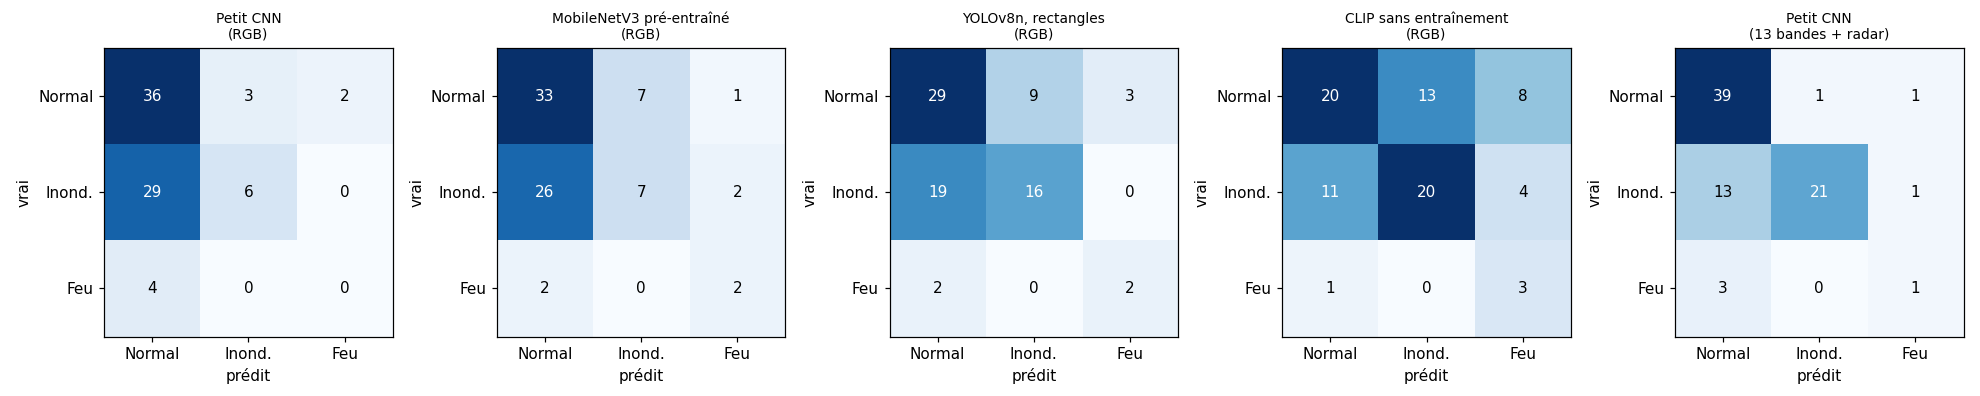
\includegraphics[width=\linewidth]{img/confusions.png}
\end{center}
\legende{Figure 5. Lignes : vérité ; colonnes : prédiction. Chiffres bruts dans docs/resultats\_modeles.json.}

% =====================================================================
\chapitre{Retour d'expérience}{Erreurs et corrections}{Les deux corrections décisives : le seuil d'alerte et la détection de l'inconnu.}
% =====================================================================

\begin{methode}[title={\cardtitle{Données}}]
\begin{itemize}[leftmargin=1.2em,itemsep=6pt]
\erreur{Le découpage officiel de Sen1Floods11 met des tuiles voisines d'un même pays en apprentissage et en test.}{découpage par pays, vérifié automatiquement.}
\erreur{La carte d'eau permanente oublie les rivières étroites, comptées comme crues.}{eau permanente élargie de 30 m, petites taches ignorées (26 tuiles corrigées).}
\erreur{Les données perm\_water ne sont pas au format annoncé (radar entre 0 et 1, tailles variables).}{conversion approximative en dB, usage limité au test des fausses alertes.}
\erreur{CaBuAr est en L2A, bien plus sombre que nos images L1C : le modèle risquait d'apprendre « image sombre = feu ».}{harmonisation linéaire bande par bande.}
\erreur{4 feux téléchargés sur 10 ne montrent aucune brûlure.}{écartés après vérification visuelle.}
\end{itemize}
\end{methode}

\begin{methode}[title={\cardtitle{Téléchargement et code}}]
\begin{itemize}[leftmargin=1.2em,itemsep=6pt]
\erreur{Téléchargements Copernicus : pannes serveur, radar sans bande VH, relief absent au-delà de 60° N, erreur SSL.}{nouvelles tentatives automatiques, fenêtres de dates successives, relief Copernicus, certificats Windows.}
\erreur{La bibliothèque \texttt{datasets} ne lit plus CaBuAr, et la lecture à distance est trop lente.}{téléchargement direct du fichier HDF5 (5,9 Go).}
\erreur{Un fichier tronqué après une coupure de connexion.}{écriture dans un fichier temporaire puis renommage, et vérification de lisibilité.}
\erreur{Les contrôles de format acceptaient un radar non converti en dB et rejetaient des tuiles pour quelques pixels négatifs.}{règles corrigées et testées sur 7 types d'entrées corrompues.}
\end{itemize}
\end{methode}

\begin{methode}[title={\cardtitle{Modèles}}]
\begin{itemize}[leftmargin=1.2em,itemsep=6pt]
\erreur{Une règle simple en RGB alerte sur 100\,\% des tuiles normales.}{modèles qui lisent la forme (CNN, YOLO), comparés à l'image complète.}
\erreur{56\,\% de fausses alertes sur le test.}{seuil d'alerte réglé sur la validation : 5\,\%.}
\erreur{Le score « énergie » fait pire que le hasard pour l'inconnu, car le bruit rend le modèle sûr de lui.}{distance de Mahalanobis, AUROC 1,00.}
\erreur{MobileNet perd la moitié de son F1 en INT8.}{modèle retenu : le petit CNN, sans perte en INT8.}
\end{itemize}
\end{methode}

\begin{center}
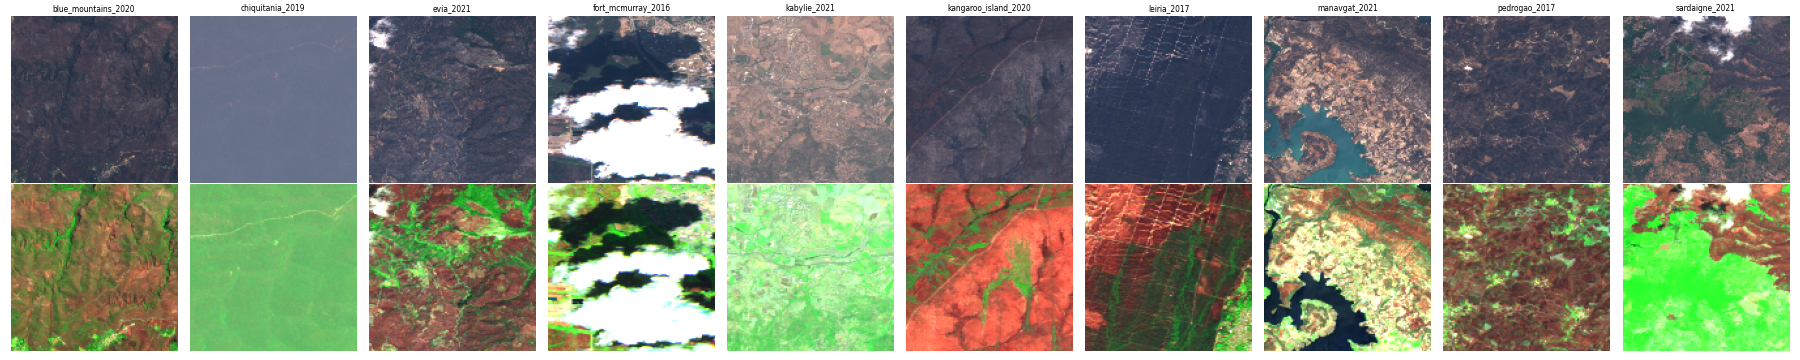
\includegraphics[width=\linewidth]{img/feux_copernicus.png}
\end{center}
\legende{Figure 6. Les 10 feux téléchargés, en couleurs naturelles (haut) et en infrarouge (bas). Quatre ont été écartés après vérification visuelle.}

\begin{attention}
Non corrigé : en radar seul, le modèle n'alerte jamais. Il n'est jamais assez sûr pour dépasser le seuil.
\end{attention}

% =====================================================================
\chapitre{Démonstration}{L'outil en action}{Trois façons de le tester sur des tuiles jamais vues.}
% =====================================================================

\begin{itemize}
\item \textbf{Vidéo} de 45 secondes (\texttt{one\_look\_demo.mp4}) : pour chaque tuile, l'image RGB, l'image infrarouge, la vérité et la décision des deux modèles.
\item \textbf{Application dans le navigateur} : \texttt{python src/demo.py}, puis ouvrir \texttt{http://127.0.0.1:7860}.
\item \textbf{Ligne de commande}, avec le code qui tournerait à bord :
\end{itemize}

\begin{codebox}
\textcolor{ink2}{\$} python src/predict.py -{}-s2 Sri-Lanka\_649970\_S2Hand.tif -{}-s1 Sri-Lanka\_649970\_S1Hand.tif\\
\textcolor{eau}{décision : INONDATION}\quad NORMAL 0,034 · INONDATION 0,963 · FEU 0,003\par\medskip
\textcolor{ink2}{\$} python src/predict.py -{}-s2 inc\_mine\_atacama\_S2.tif -{}-s1 inc\_mine\_atacama\_S1.tif\\
\textcolor{syspurple}{décision : INCONNU}\quad image trop différente des données connues (distance 961, seuil 337)
\end{codebox}

\begin{center}
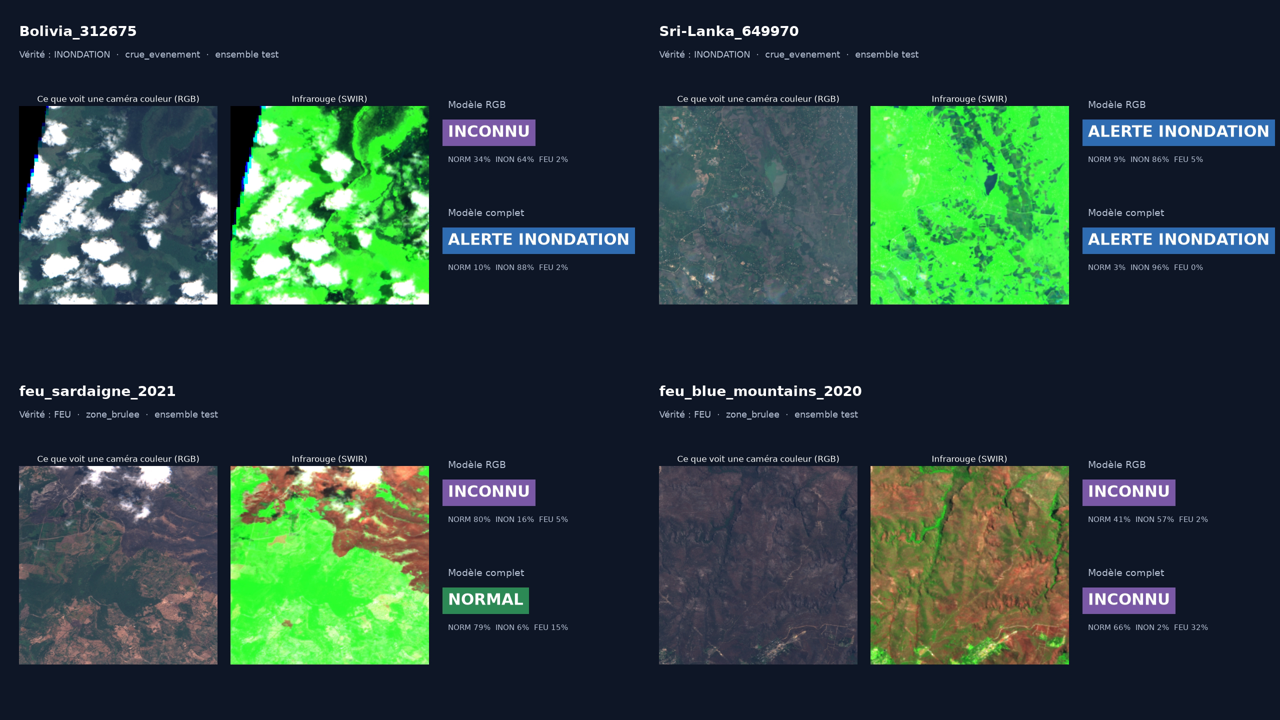
\includegraphics[width=0.57\linewidth]{img/demo_1.png}
\end{center}
\legende{Figure 7. Inondations détectées en Bolivie et au Sri Lanka ; feux de Sardaigne et d'Australie manqués.}

\begin{center}
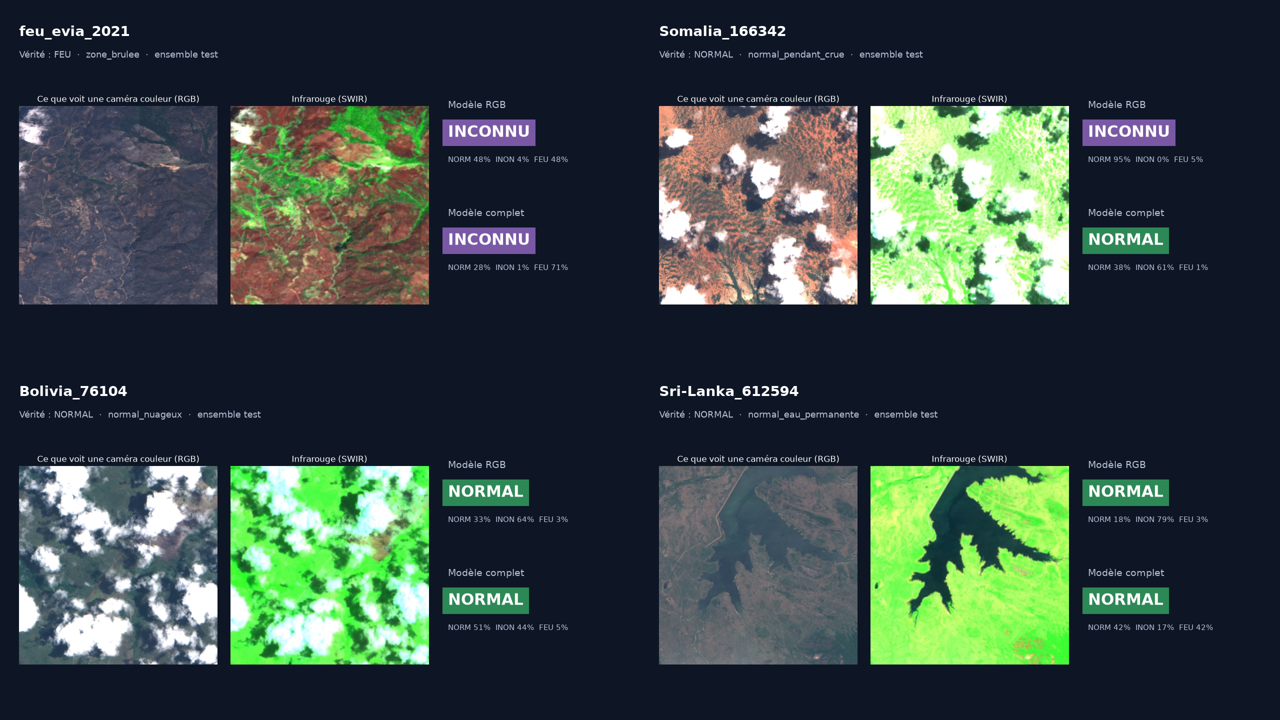
\includegraphics[width=0.57\linewidth]{img/demo_2.png}
\end{center}
\legende{Figure 8. Feu de Grèce signalé inconnu ; tuiles normales, dont un réservoir, bien classées.}

% =====================================================================
\chapitre{Bilan}{Limites et suite}{Ce qui ne marche pas encore, et ce qui viendrait ensuite.}
% =====================================================================

\begin{attention}
\begin{itemize}[leftmargin=1.2em]
\item En radar seul, le modèle n'alerte jamais : il faudrait un modèle dédié au radar, avec son propre seuil.
\item 40\,\% des inondations sont manquées, le prix d'un seuil réglé pour limiter les fausses alertes.
\item Il n'y a que 4 feux dans le test, donc les résultats sur les feux restent très incertains ; CaBuAr ne couvre que la Californie.
\item Les étiquettes sont imparfaites : la crue dépend de la carte d'eau permanente, et les scènes Copernicus sont étiquetées d'après leur date.
\end{itemize}
\end{attention}

\begin{definition}[title={\cardtitle{Suite}}]
Ajouter des feux hors Californie, entraîner un modèle dédié au radar, et tester le modèle sur une vraie carte embarquée.
\end{definition}

\begin{complt}
Outils : Python, PyTorch, rasterio, scikit-learn, ONNX Runtime, Ultralytics, Hugging Face, openEO. Modèles pré-entraînés : MobileNetV3-small (ImageNet), YOLOv8n (COCO), CLIP ViT-B/32. Le code et la documentation ont été écrits avec l'aide d'un assistant IA (Claude) ; les choix et les vérifications ont été validés par l'auteur.
\end{complt}

\end{document}
